\documentclass[10pt,mathserif]{beamer}

% ------------------------------------------------------------------------
% Packages
% ------------------------------------------------------------------------
\usepackage{amsmath}
\usepackage{tabularx}

% ------------------------------------------------------------------------
% Macros
% ------------------------------------------------------------------------
%~~~~~~~~~~~~~~~
% List shorthand
%~~~~~~~~~~~~~~~
\newcommand{\BIT}{\begin{itemize}}
\newcommand{\EIT}{\end{itemize}}
\newcommand{\BNUM}{\begin{enumerate}}
\newcommand{\ENUM}{\end{enumerate}}
%~~~~~~~~~~~~~~~
% Text with quads around it
%~~~~~~~~~~~~~~~
\newcommand{\qtext}[1]{\quad\text{#1}\quad}
%~~~~~~~~~~~~~~~
% Shorthand for math formatting
%~~~~~~~~~~~~~~~
\newcommand\mbb[1]{\mathbb{#1}}
\newcommand\mbf[1]{\mathbf{#1}}
\def\mc#1{\mathcal{#1}}
\def\mrm#1{\mathrm{#1}}
%~~~~~~~~~~~~~~~
% Common sets
%~~~~~~~~~~~~~~~
\def\reals{\mathbb{R}} % Real number symbol
\def\integers{\mathbb{Z}} % Integer symbol
\def\rationals{\mathbb{Q}} % Rational numbers
\def\naturals{\mathbb{N}} % Natural numbers
\def\complex{\mathbb{C}} % Complex numbers
\def\simplex{\mathcal{S}} % Simplex
%~~~~~~~~~~~~~~~
% Common functions
%~~~~~~~~~~~~~~~
\renewcommand{\exp}[1]{\operatorname{exp}\left(#1\right)} % Exponential
\def\indic#1{\mbb{I}\left({#1}\right)} % Indicator function
\providecommand{\maximize}{\mathop\mathrm{maximize}} % Defining math symbols
\providecommand{\minimize}{\mathop\mathrm{minimize}}
\providecommand{\argmax}{\mathop\mathrm{arg max}}
\providecommand{\argmin}{\mathop\mathrm{arg min}}
\providecommand{\arccos}{\mathop\mathrm{arccos}}
\providecommand{\asinh}{\mathop\mathrm{asinh}}
\providecommand{\dom}{\mathop\mathrm{dom}} % Domain
\providecommand{\range}{\mathop\mathrm{range}} % Range
\providecommand{\diag}{\mathop\mathrm{diag}}
\providecommand{\tr}{\mathop\mathrm{tr}}
\providecommand{\abs}{\mathop\mathrm{abs}}
\providecommand{\card}{\mathop\mathrm{card}}
\providecommand{\sign}{\mathop\mathrm{sign}}
\def\rank#1{\mathrm{rank}({#1})}
\def\supp#1{\mathrm{supp}({#1})}
%~~~~~~~~~~~~~~~
% Common probability symbols
%~~~~~~~~~~~~~~~
\def\E{\mathbb{E}} % Expectation symbol
\def\Earg#1{\E\left[{#1}\right]}
\def\Esubarg#1#2{\E_{#1}\left[{#2}\right]}
\def\P{\mathbb{P}} % Probability symbol
\def\Parg#1{\P\left({#1}\right)}
\def\Psubarg#1#2{\P_{#1}\left[{#2}\right]}
\def\Cov{\mrm{Cov}} % Covariance symbol
\def\Corr{\mrm{Corr}} % Covariance symbol
\def\Covarg#1{\Cov\left[{#1}\right]}
\def\Covsubarg#1#2{\Cov_{#1}\left[{#2}\right]}
\def\Corrsubarg#1#2{\Corr_{#1}\left[{#2}\right]}
\def\Var{\mrm{Var}}
\def\Vararg#1{\Var\left(#1\right)}
\def\Varsubarg#1#2{\Var_{#1}\left(#2\right)}
\newcommand{\family}{\mathcal{P}} % probability family
\newcommand{\eps}{\epsilon}
\def\absarg#1{\left|#1\right|}
\def\msarg#1{\left(#1\right)^{2}}
\def\logarg#1{\log\left(#1\right)}
%~~~~~~~~~~~~~~~
% Distributions
%~~~~~~~~~~~~~~~
\def\Gsn{\mathcal{N}}
\def\Ber{\textnormal{Ber}}
\def\Bin{\textnormal{Bin}}
\def\Unif{\textnormal{Unif}}
\def\Mult{\textnormal{Mult}}
\def\Cat{\textnormal{Cat}}
\def\Gam{\textnormal{Gam}}
\def\InvGam{\textnormal{InvGam}}
\def\NegMult{\textnormal{NegMult}}
\def\Dir{\textnormal{Dir}}
\def\Lap{\textnormal{Laplace}}
\def\Bet{\textnormal{Beta}}
\def\Poi{\textnormal{Poi}}
\def\HypGeo{\textnormal{HypGeo}}
\def\GEM{\textnormal{GEM}}
\def\BP{\textnormal{BP}}
\def\DP{\textnormal{DP}}
\def\BeP{\textnormal{BeP}}
%~~~~~~~~~~~~~~~
% Theorem-like environments
%~~~~~~~~~~~~~~~

%-----------------------
% Probability sets
%-----------------------
\newcommand{\X}{\mathcal{X}}
\newcommand{\Y}{\mathcal{Y}}
\newcommand{\D}{\mathcal{D}}
\newcommand{\Scal}{\mathcal{S}}
%-----------------------
% vector notation
%-----------------------
\newcommand{\bx}{\mathbf{x}}
\newcommand{\by}{\mathbf{y}}
\newcommand{\bt}{\mathbf{t}}
\newcommand{\xbar}{\overline{x}}
\newcommand{\Xbar}{\overline{X}}
\newcommand{\tolaw}{\xrightarrow{\mathcal{L}}}
\newcommand{\toprob}{\xrightarrow{\mathbb{P}}}
\newcommand{\laweq}{\overset{\mathcal{L}}{=}}
\newcommand{\F}{\mathcal{F}}

\usepackage{graphicx,amsmath,amssymb}
\usepackage{listings}
\lstset{language=Python}

%% \input defs.tex

%% formatting
\setbeamertemplate{navigation symbols}{}
\usecolortheme[rgb={0.13,0.28,0.59}]{structure}
\setbeamertemplate{itemize subitem}{--}
\setbeamertemplate{frametitle} {
	\begin{center}
	  {\large\bf \insertframetitle}
	\end{center}
}

\newcommand\footlineon{
  \setbeamertemplate{footline} {
    \begin{beamercolorbox}[ht=2.5ex,dp=1.125ex,leftskip=.8cm,rightskip=.6cm]{structure}
      \footnotesize \insertsection
      \hfill
      {\insertframenumber}
    \end{beamercolorbox}
    \vskip 0.45cm
  }\begin{figure}[ht]
  \centering
  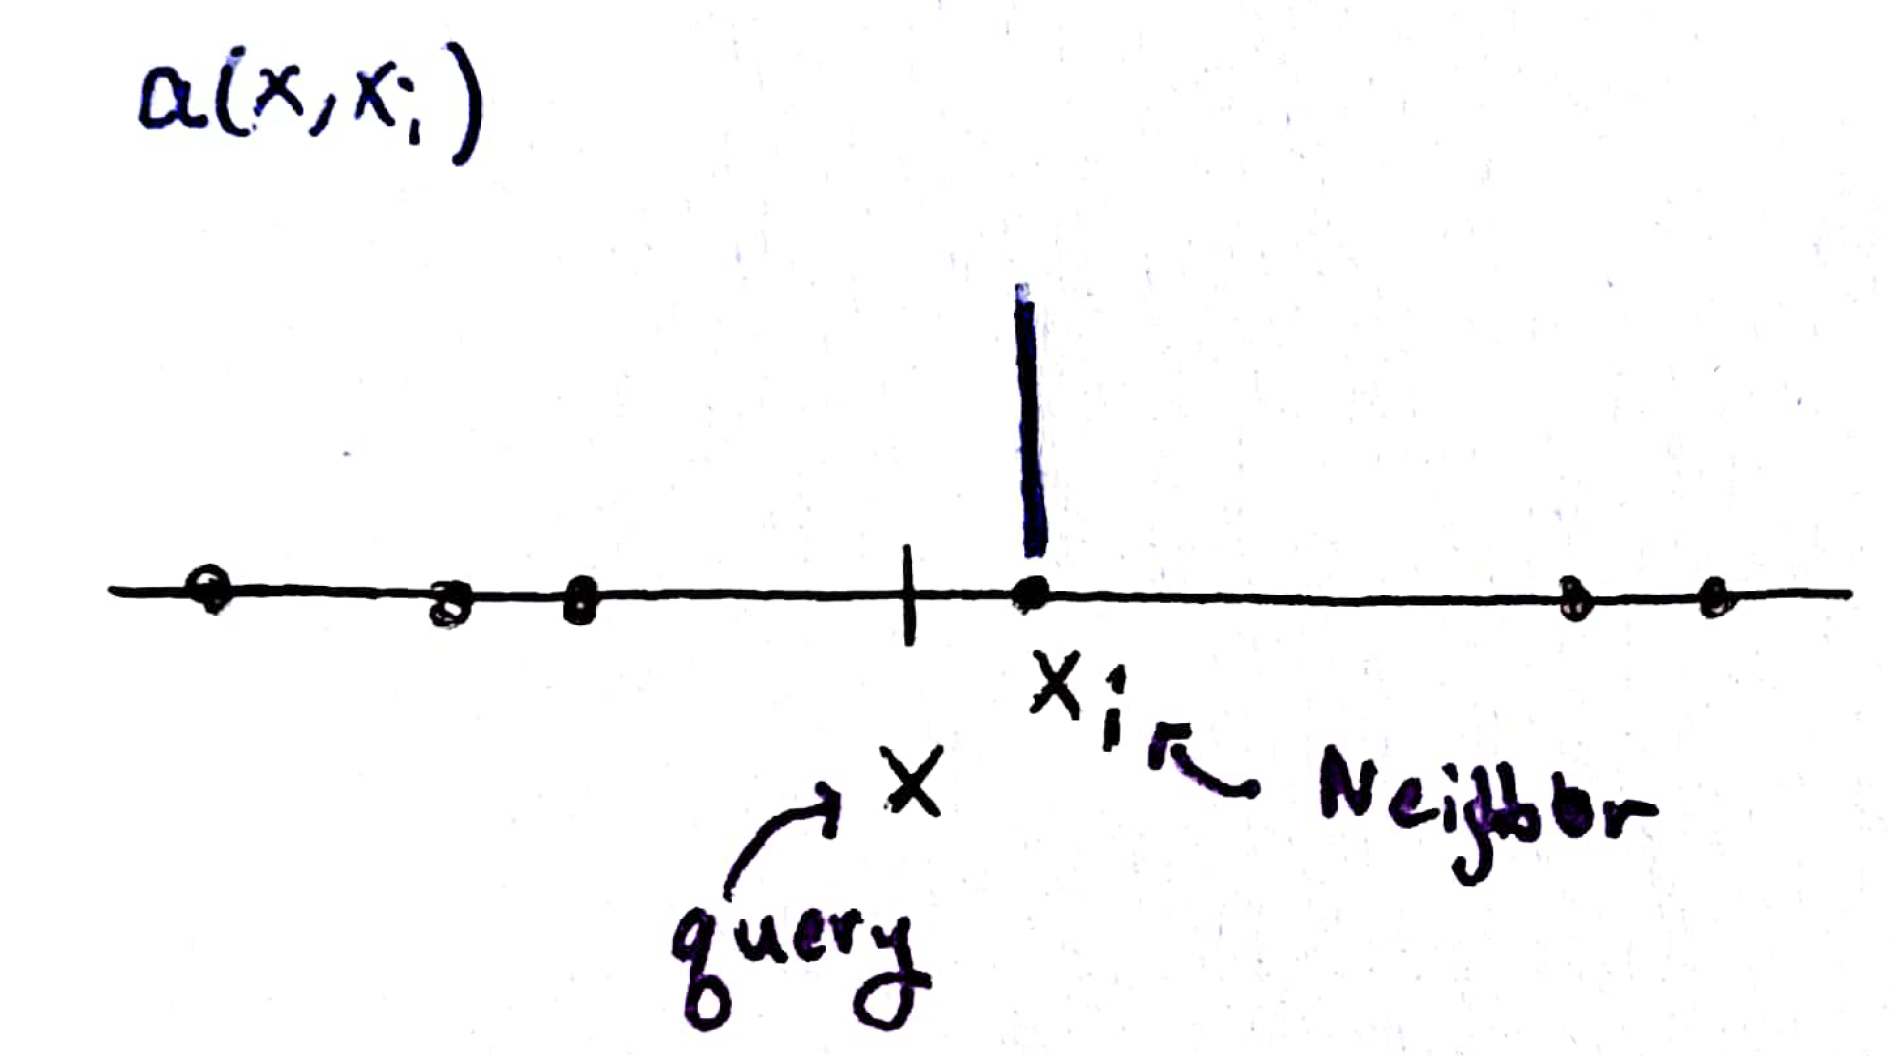
\includegraphics[width=0.7\paperwidth]{figure/hard_a_fun}
  \caption{\label{fig:hard_a_fun} }
\end{figure}

}
\footlineon

\AtBeginSection
{
	\begin{frame}<beamer>
		\frametitle{Outline}
		\tableofcontents[currentsection,currentsubsection]
	\end{frame}
}

%% begin presentation

\title{\large \bfseries Generative Adversarial Networks}

\author{Kris Sankaran\\[3ex]
Mila}

\date{\today}

\begin{document}

\frame{
  \thispagestyle{empty}
  \titlepage
}

\section{Introduction}

\begin{frame}
  \frametitle{Learning Objectives}
 \begin{itemize}
  \item Understand basic adversarial setup
  \item Density estimation view of GANs
  \item Stabilize training: WGAN
  \item Real-world applications
 \end{itemize}
\end{frame}

\begin{frame}
\begin{itemize}
\item GANs are popular ways to generate images
\end{itemize}
\begin{figure}[ht]
  \centering
  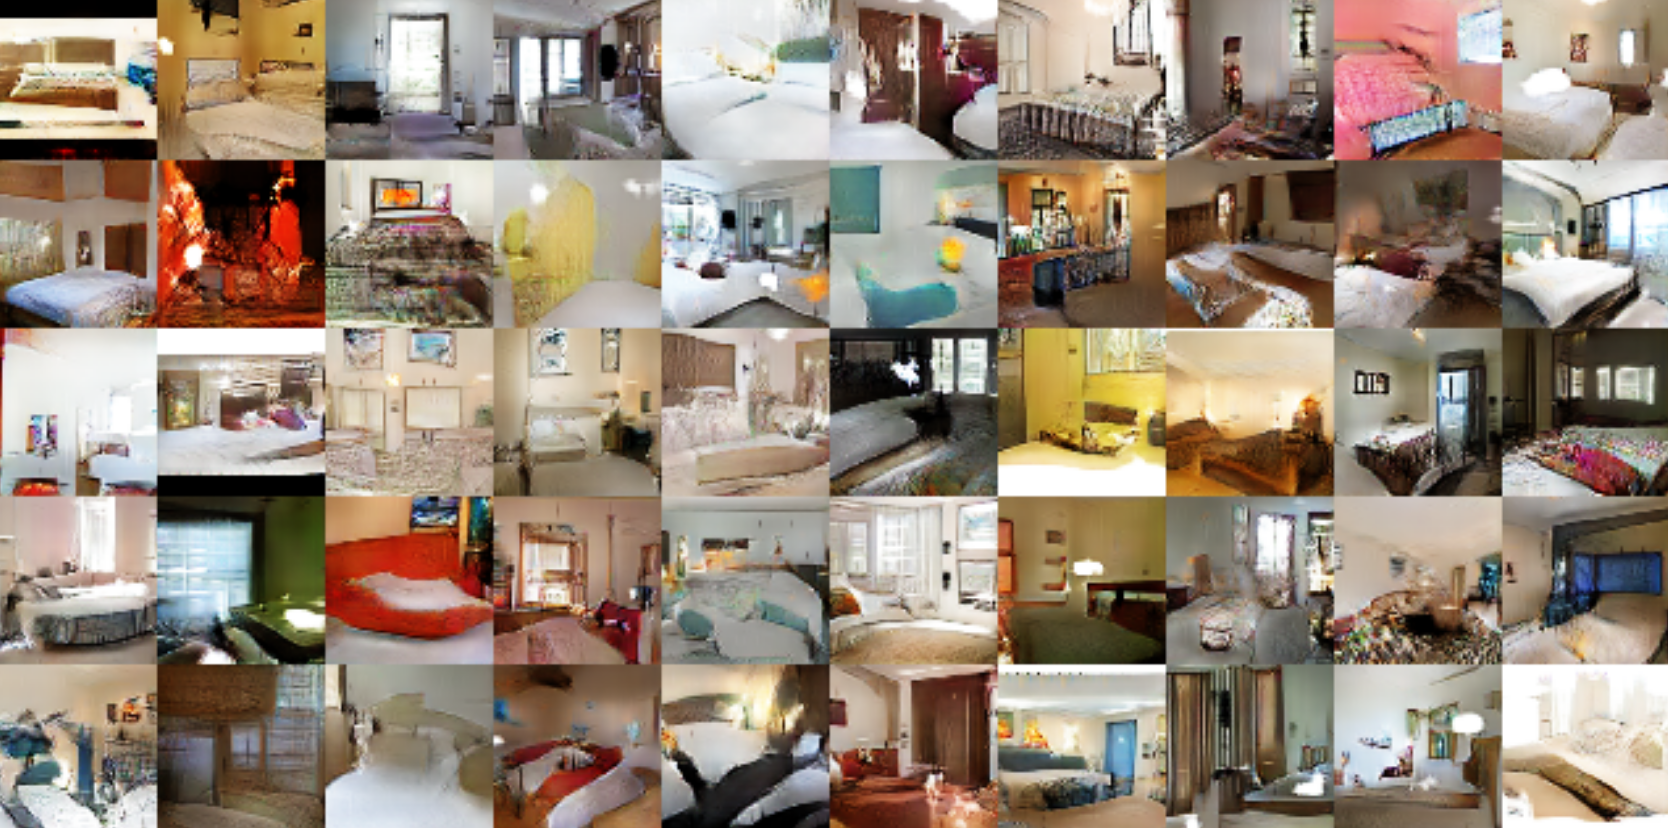
\includegraphics[width=0.7\paperwidth]{figure/gan_example}
  \caption{Example GAN samples. \label{fig:gan_example} }
\end{figure}
\end{frame}

\begin{frame}
\begin{itemize}
\item It's better to think of them as learning how to sample from probability
  densities $p\left(x\right)$
\item For $32 \times 32$ images, $p\left(x\right)$ is a distribution in
  1024-dimensional space
\item What's exciting is that they are \textit{implicit} probability models
\end{itemize}
\begin{figure}[ht]
  \centering
  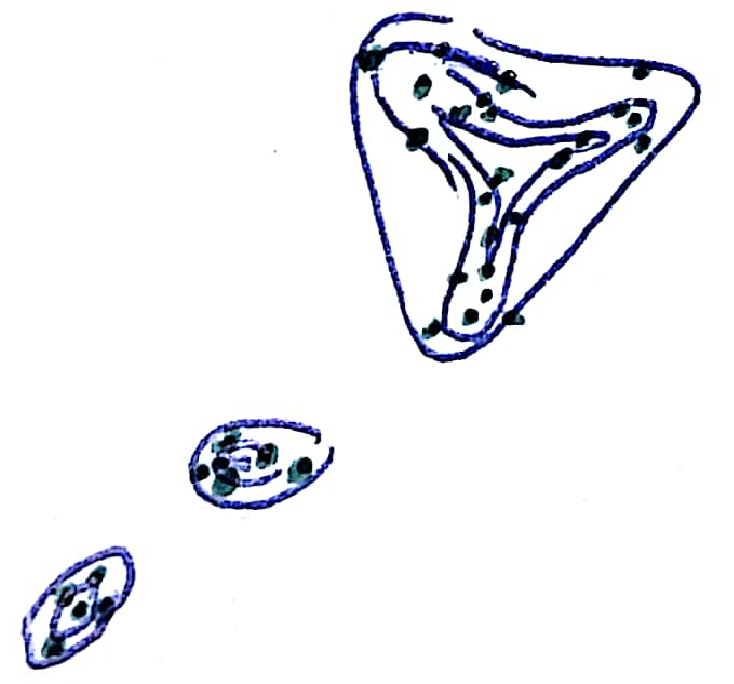
\includegraphics[width=0.7\paperwidth]{figure/gan_density}
  \caption{\label{fig:gan_density} }
\end{figure}
\end{frame}

\begin{frame}
\begin{itemize}
\item Interpolations are just sampling along lines in a probability density
\end{itemize}
\begin{figure}[ht]
  \centering
  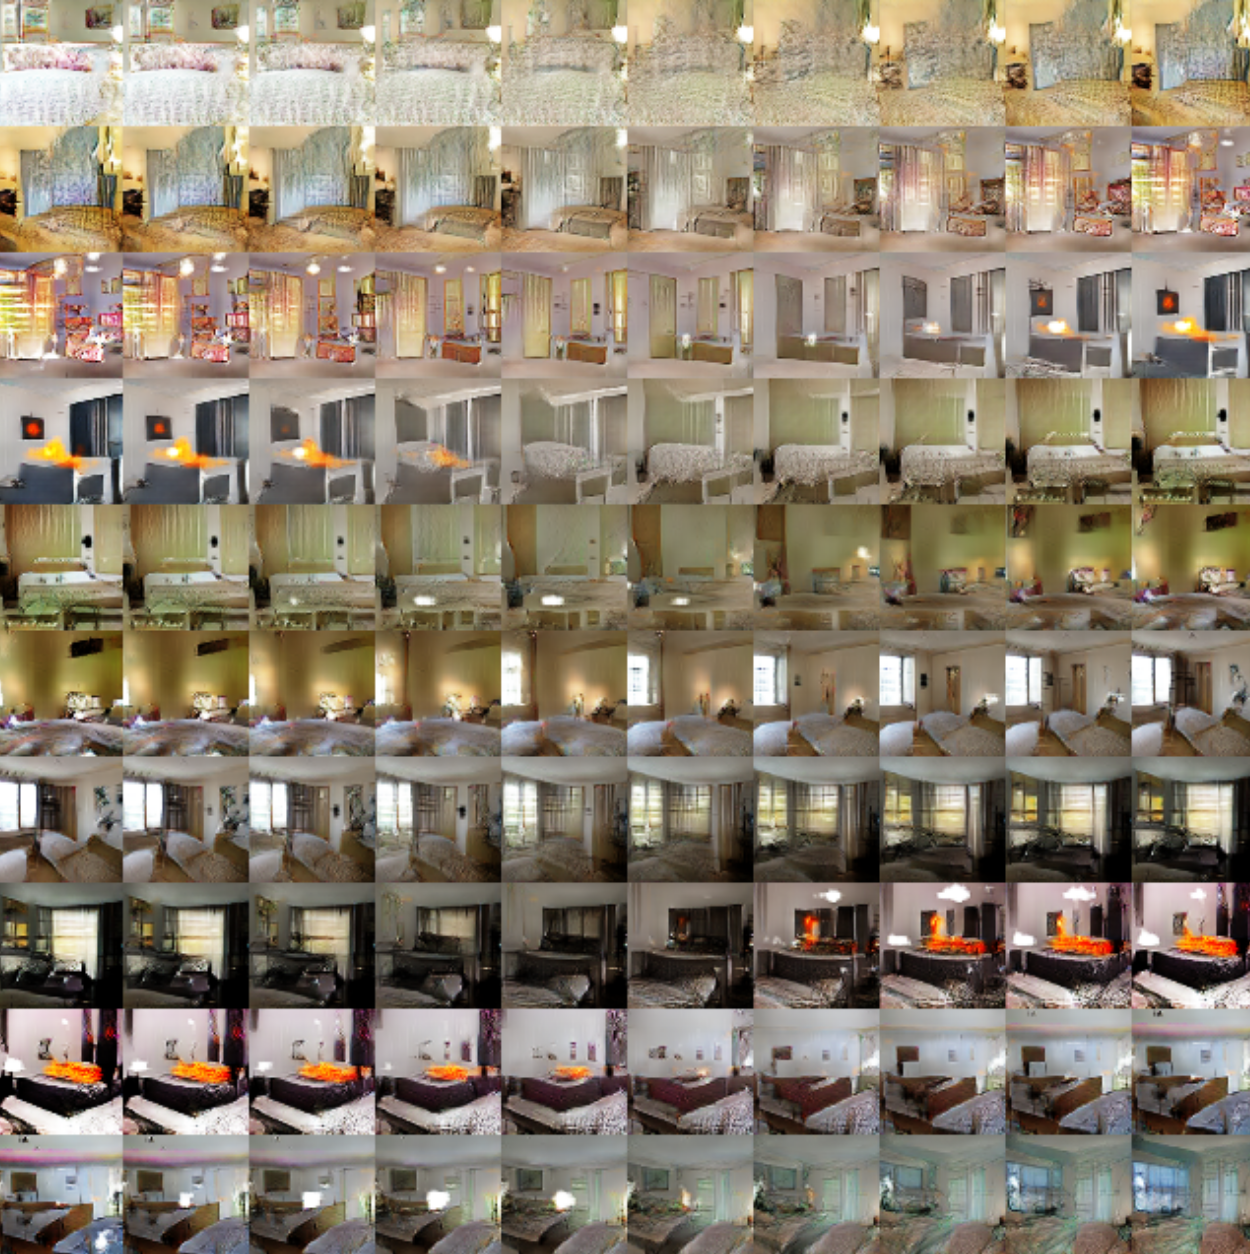
\includegraphics[width=0.7\paperwidth]{figure/gans_interpolations}
  \caption{\label{fig:gan_interpolations} }
\end{figure}
\end{frame}

\begin{frame}
\begin{itemize}
  \item Interpolations are just sampling along lines in a probability density
\end{itemize}
\begin{figure}[ht]
  \centering
  \includegraphics[width=0.7\paperwidth]{figure/gan_interpolations_density}
  \caption{\label{fig:gan_interpolations_density} }
\end{figure}
\end{frame}

\section{Formulation}

\begin{frame}
  \frametitle{Formulation}
 \begin{itemize}
 \item How to transform (say, uniform) noise $z$ into arbitrary distributions?
 \item Idea: Use a neural network $G$
 \item $z \rightarrow G\left(z\right)$
 \end{itemize}
\begin{figure}[ht]
  \centering
  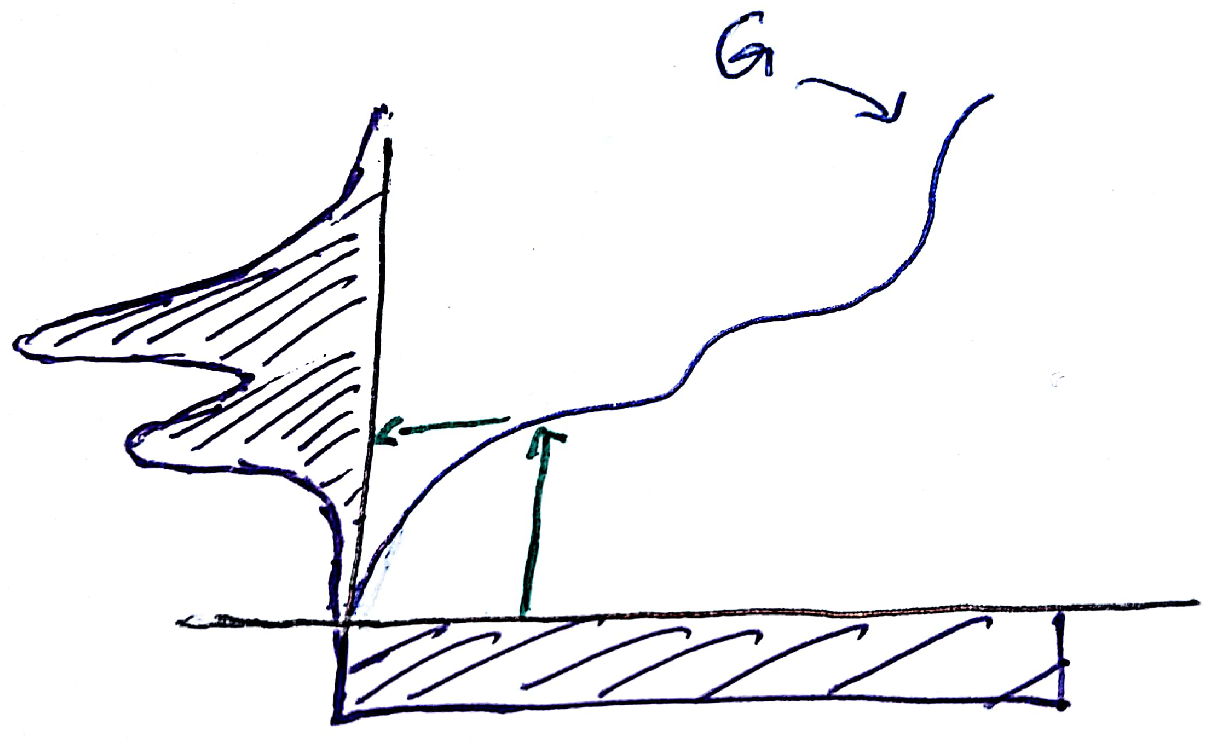
\includegraphics[width=0.7\paperwidth]{figure/sample_transformation}
  \caption{\label{fig:sample_transformation} }
\end{figure}
\end{frame}

\begin{frame}
  \frametitle{Formulation}
 \begin{itemize}
 \item How to learn a transformation to match observed data?
 \item Idea: Use another neural network! Call it $D$.
 \item This is pretty different from usual likelihood-based views
   \begin{itemize}
   \item (there are connections though)
   \end{itemize}
 \end{itemize}
\begin{figure}[ht]
  \centering
  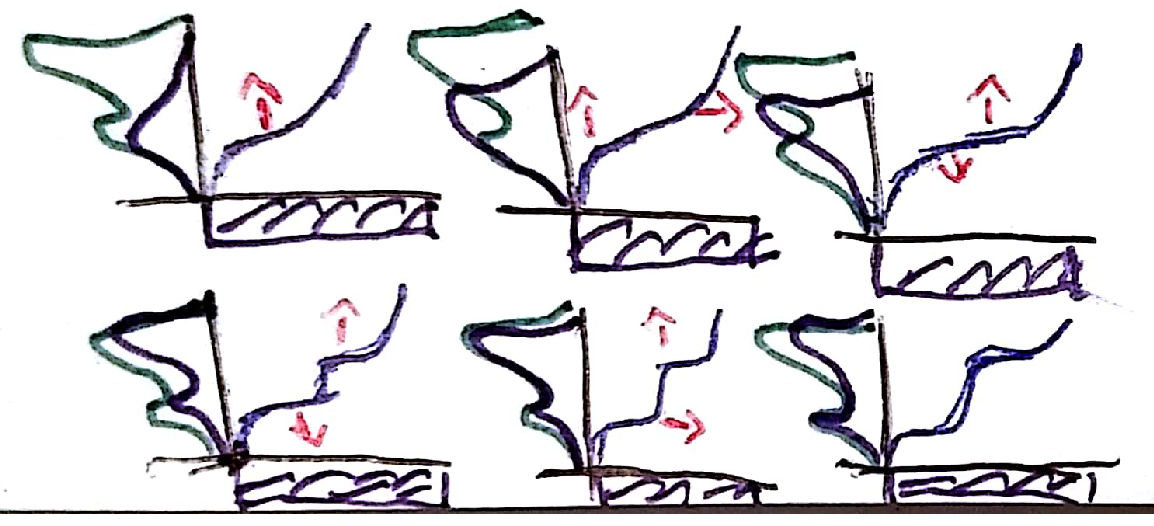
\includegraphics[width=0.7\paperwidth]{figure/discriminator_transformation}
  \caption{\label{fig:discriminator_transformation} }
\end{figure}
\end{frame}

\begin{frame}
\frametitle{Objective Function}
 \begin{itemize}
   \item How should $D$ guide these updates?
   \item Objective function
     \begin{align*}
       \min_{G}\max_{D} V\left(D, G\right) = \Esubarg{p_{\text{data}}}{D\left(x\right)} + \Esubarg{p\left(z\right)}{\log\left(1 - D\left(G\left(z\right)\right)\right)}
     \end{align*}
   \item Alternate gradient steps, first update $D$, then $G$, then $D$, ...
\begin{itemize}
\item $D$ is encouraged to be large on $x$ and small on $G\left(z\right)$, so
  that the objective gets large
\item $G$ is encouraged to make $D$ assign values near 1 to samples $G\left(z\right)$, so that the objective gets small
\end{itemize}
 \end{itemize}
\begin{figure}[ht]
  \centering
  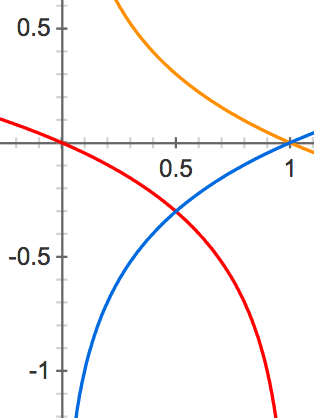
\includegraphics[width=0.7\paperwidth]{figure/gan_objectives}
  \caption{The green line is $\log\left(x\right)$ and the purple is $\log\left(1
    - x\right)$, on the range $\left[0, 1\right]$ of possible
    probabilities. \label{fig:gan_objectives} }
\end{figure}
\end{frame}

\begin{frame}
  \frametitle{GAN Lab}
 \begin{itemize}
   \url{https://poloclub.github.io/ganlab/}
 \end{itemize}
\begin{figure}[ht]
  \centering
  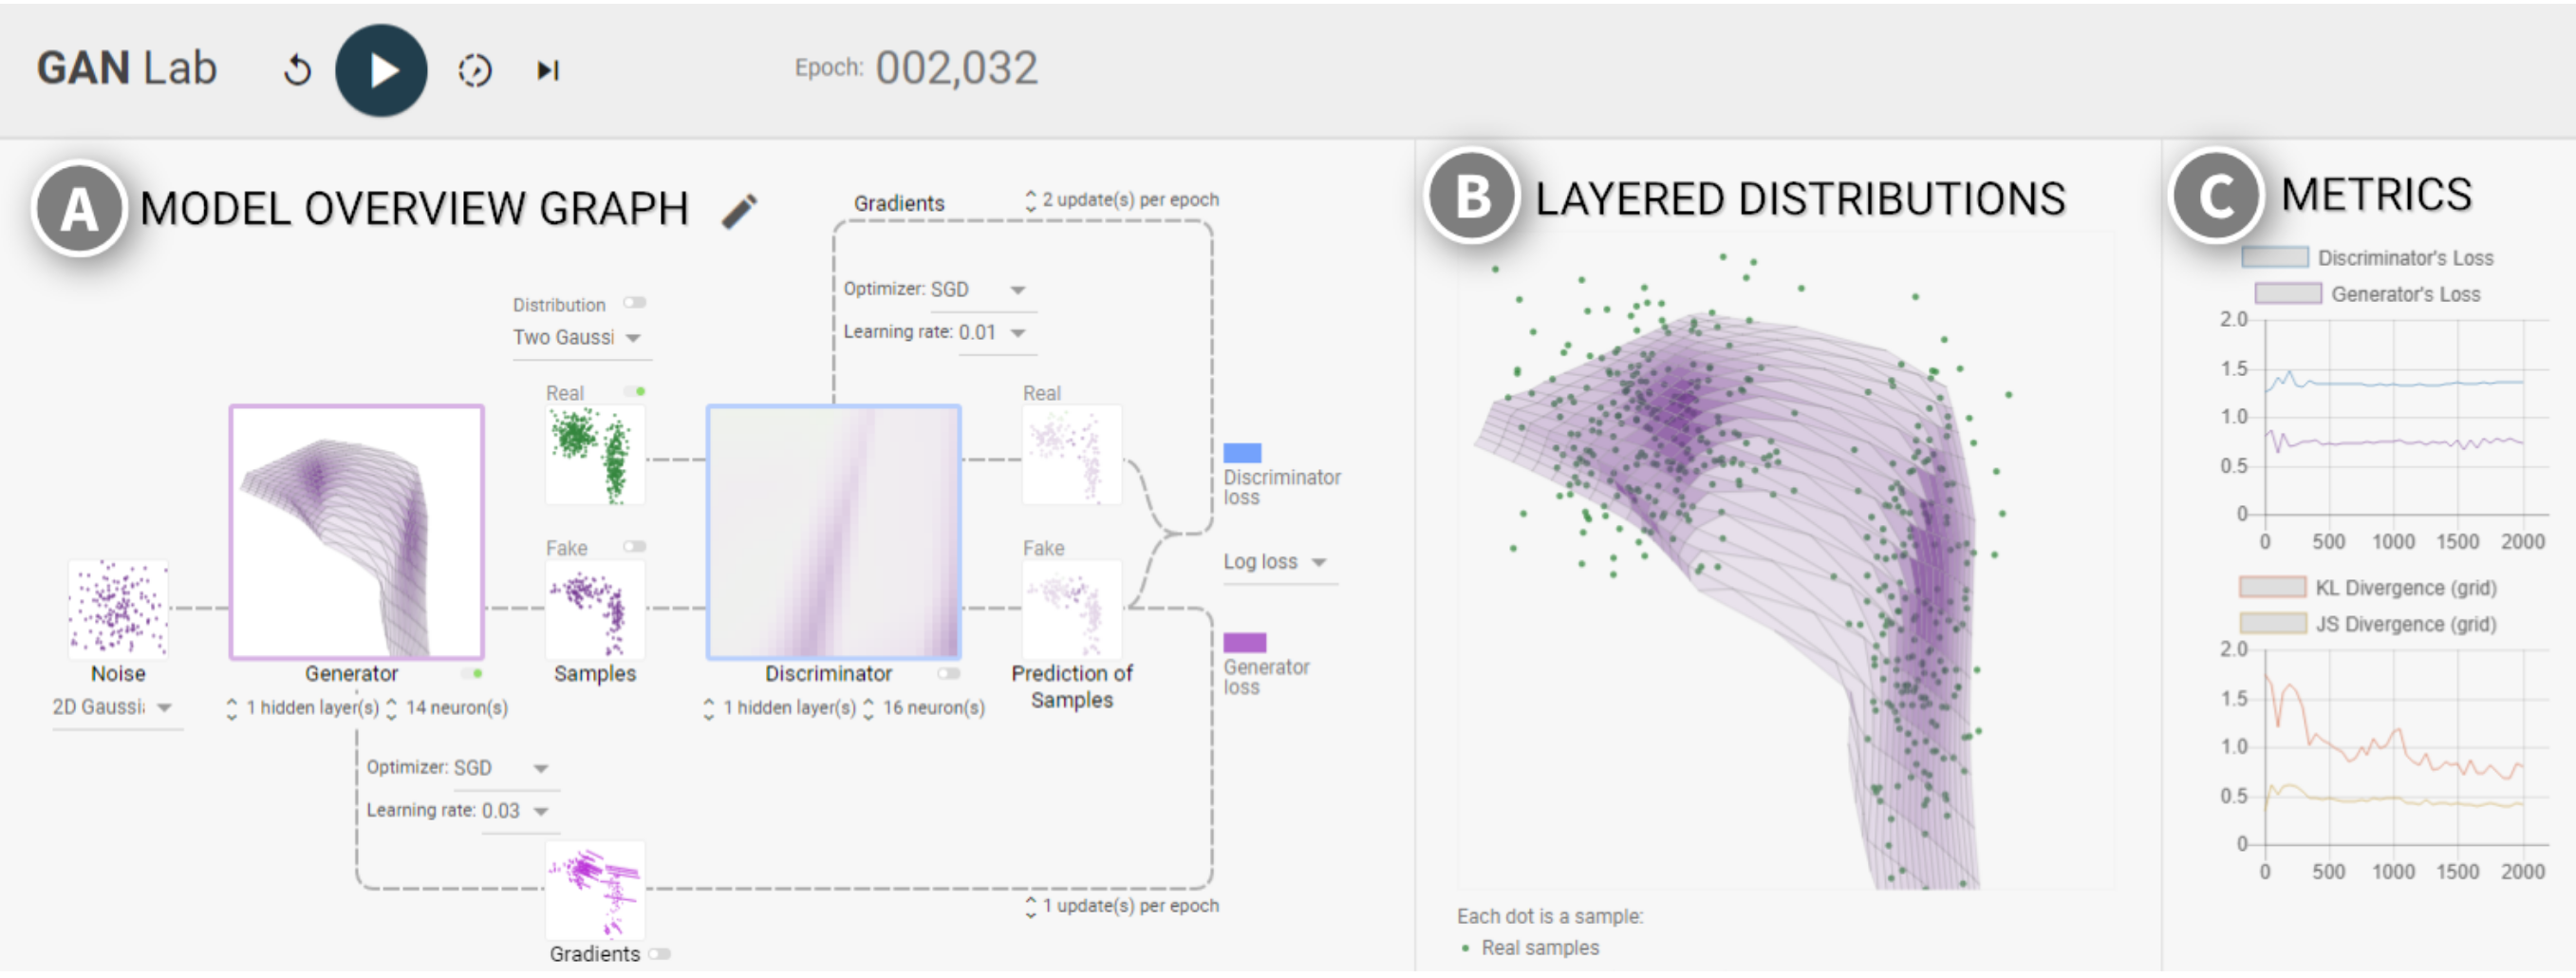
\includegraphics[width=0.7\paperwidth]{figure/ganlab}
  \caption{A visualization of the whole process, on a few different toy
    datasets. \label{fig:ganlab} }
\end{figure}
\end{frame}

\section{Perspectives}
\label{sec:perspectives}

\begin{frame}
  \frametitle{Training difficulties}
 \begin{itemize}
 \item GANs have a bad reputation for being finnicky to train
 \item If the discriminator is ``too strong,'' it might not communicate useful
   information
 \end{itemize}
\begin{figure}[ht]
  \centering
  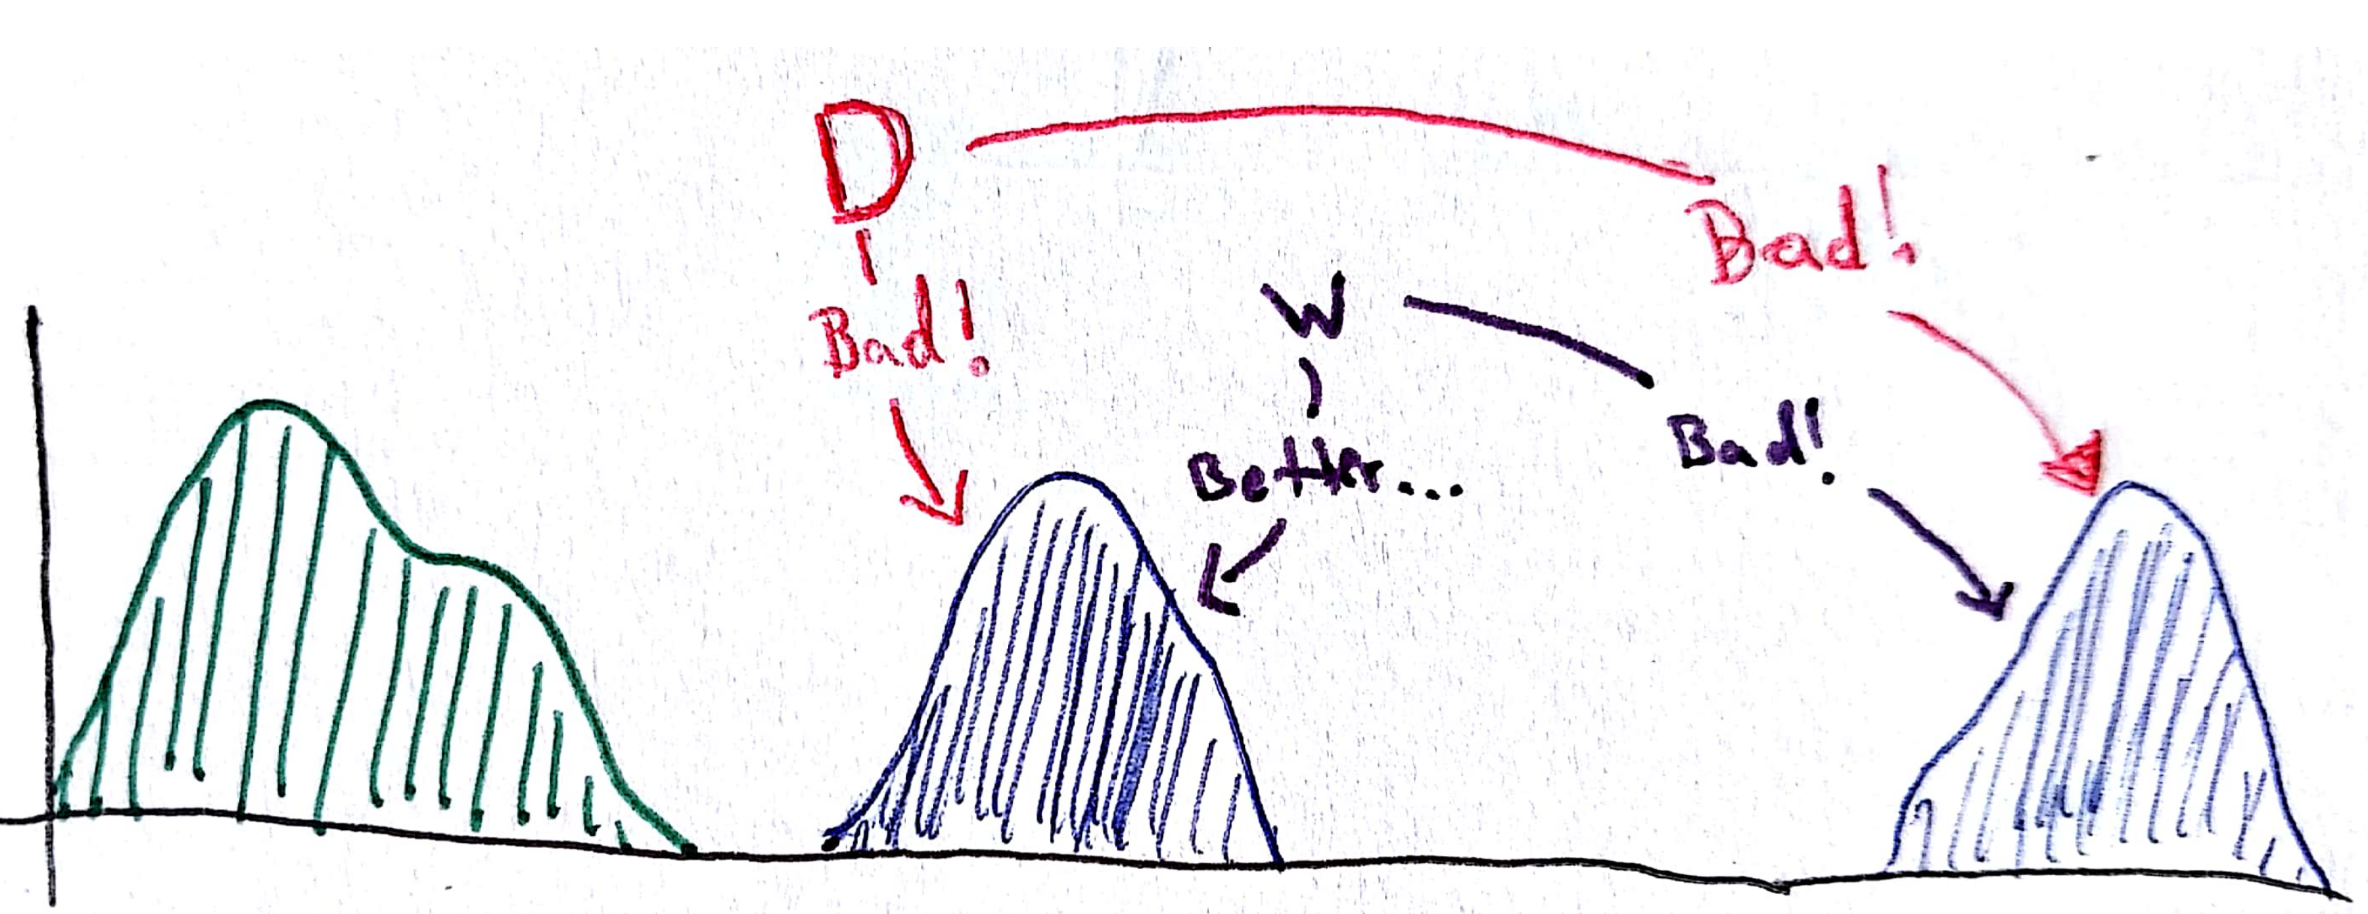
\includegraphics[width=0.7\paperwidth]{figure/alternative_critic}
  \caption{We would like a critic that tells the generator when it's getting
    closer, even when it's obviously different from the
    target. \label{fig:alternative_critic} }
\end{figure}
\end{frame}

\begin{frame}
  \frametitle{Wasserstein GAN}
 \begin{itemize}
 \item Formalize this idea using distances $d\left(\P_1, \P_2\right)$ between
   probability distributions
 \item Distances between Gaussians $\Gsn\left(\mu_1, 1\right)$ and
   $\Gsn\left(\mu_2, 1\right)$.
\begin{itemize}
  \item KL-divergence: $1 + \frac{1}{2} \left(\mu_2 - \mu_1\right)^2$
  \item Wasserstein distance:
\end{itemize}
\item Wasserstein distance tells us something even when they are far away!
\item Effect is even more pronounced in very-high dimensions
 \end{itemize}
\end{frame}

\begin{frame}
  \frametitle{Wasserstein Objective}
 \begin{itemize}
 \item Wasserstein distance between data $X$ and generated $\tilde{X}$
   distributions is defined by
   \begin{align*}
     d\left(\P_X, \P_\tilde{X}\right) &= \max_{\|f\|_{L} \leq 1} \Esubarg{X}{f\left(x\right)} - \Esubarg{\tilde{X}}{f\left(\tilde{x}\right)}
   \end{align*}
   where $\|f\|_{L} \leq 1$ is the set of functions whose slopes are always less
   than 1.
 \end{itemize}
\begin{figure}[ht]
  \centering
  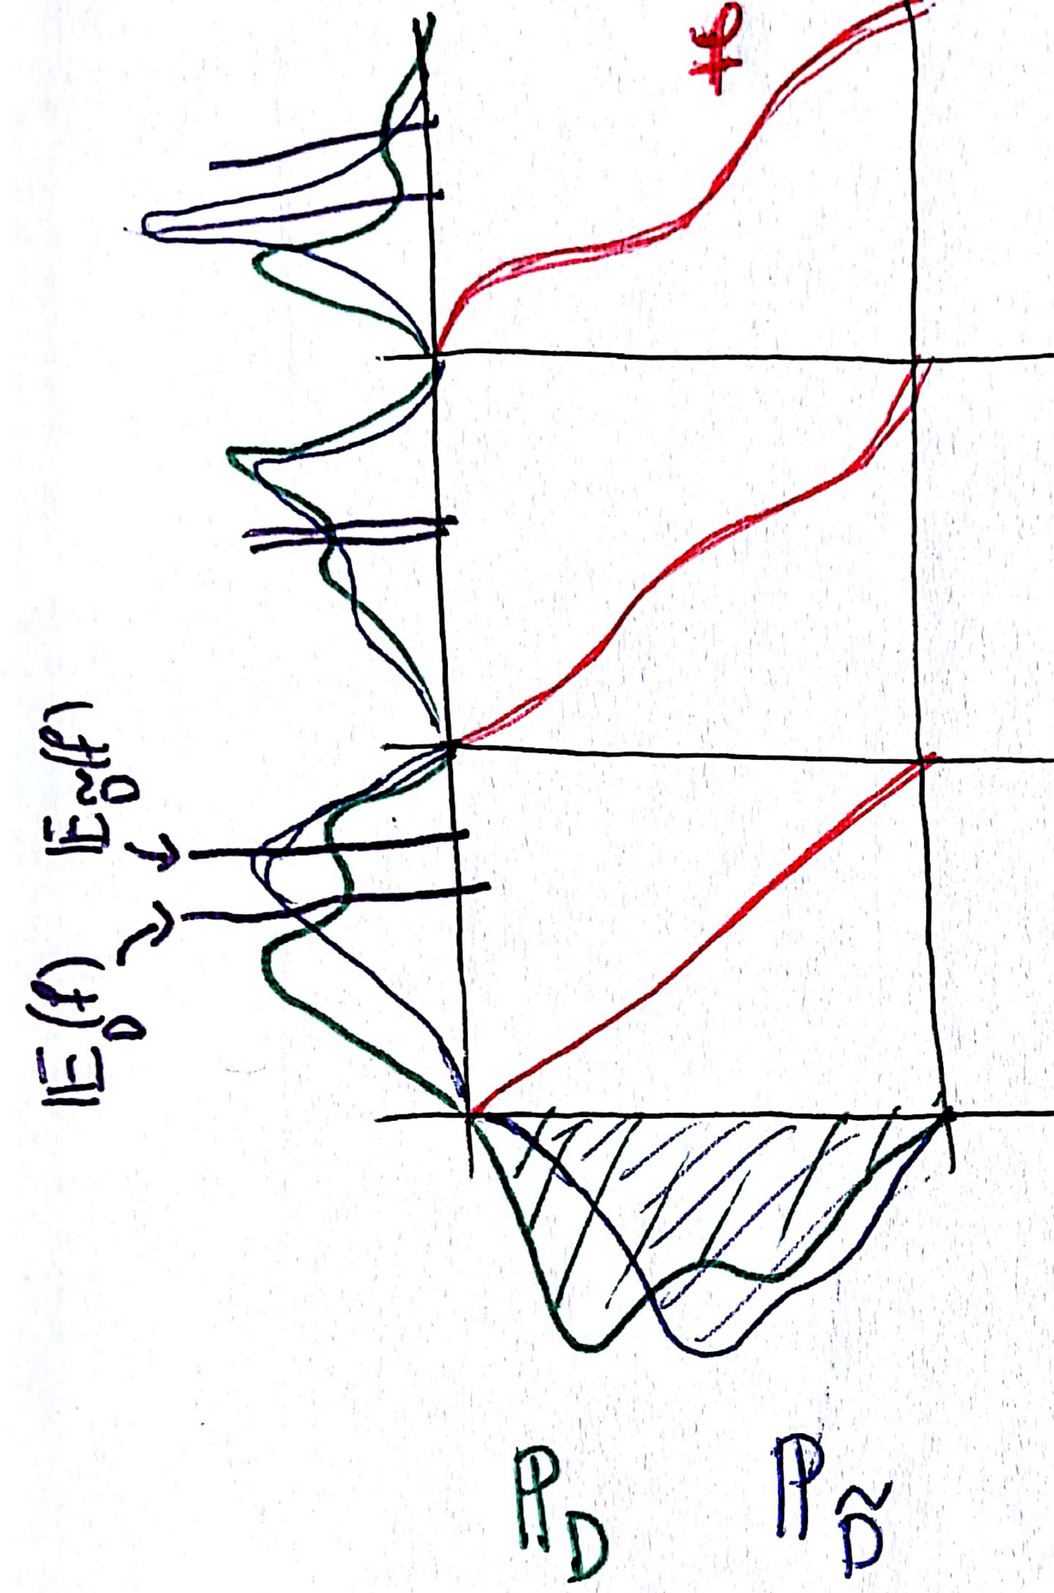
\includegraphics[width=0.7\paperwidth]{figure/wasserstein_tests}
  \caption{You can interpret the objective as computing differences in means
    after passing samples through a variety of (not too wild) test
    functions.\label{fig:wasserstein_tests} }
\end{figure}
\end{frame}

\begin{frame}
  \frametitle{Wasserstein Training}
 \begin{itemize}
 \item In terms of the transformed noise $G\left(z\right)$, this looks like
   \begin{align*}
     d\left(\P_{X}, \P_{\tilde{X}}\right) &= \max_{\|f\| \leq 1} \Esubarg{X}{f\left(x\right)} - \Esubarg{Z}{f\left(G\left(z\right))}
   \end{align*}
 \item Finding the optimal $f$ for any particular choice of $G$ is complicated...
 \item Alternatively do gradient updates
\begin{itemize}
\item Critic $f$ inches towards its maximizing value of $d\left(\P_{X},
  \P_{\tilde{X}}\right)$.
\item Generator $G$ descends towards smaller wasserstein distances
\item Constraint $\|f\|_{L} \leq 1$ maintained either by clipping or
  regularization
\end{itemize}
 \end{itemize}
\end{frame}

\begin{frame}
  \frametitle{Density Ratio Matching}
  \begin{itemize}
  \item Another useful perspective comes from thinking about density ratios.
  \end{itemize}
\end{frame}

\begin{frame}
  \frametitle{Conclusion}
\end{frame}

\end{document}
